\section{Các kỹ thuật Tối ưu và Chính quy hóa}
\label{sec:optimization_regularization_techniques}

Việc xây dựng các kiến trúc CNN ngày càng sâu hơn như ResNet hay DenseNet mới chỉ là một nửa câu chuyện. Nửa còn lại, và cũng không kém phần quan trọng, là làm thế nào để \textit{huấn luyện} những con quái vật tính toán này một cách hiệu quả. Khi các mạng nơ-ron trở nên sâu hơn và có nhiều tham số hơn, bài toán huấn luyện ngày càng trở nên khó khăn: gradient dễ dàng biến mất hoặc bùng nổ, mô hình trở nên cực kỳ nhạy cảm với cách khởi tạo trọng số, và nguy cơ quá khớp (overfitting) vào tập dữ liệu huấn luyện tăng lên theo cấp số nhân.

Để thuần hóa những mạng nơ-ron sâu này, cộng đồng nghiên cứu đã phát triển một bộ công cụ gồm các kỹ thuật tối ưu hóa và chính quy hóa (regularization) mạnh mẽ. Các kỹ thuật này không thay đổi kiến trúc cốt lõi của mạng, nhưng lại đóng vai trò như những "chất bôi trơn" và "bộ ổn định", giúp quá trình học hội tụ nhanh hơn, ổn định hơn, và quan trọng nhất, tạo ra các mô hình có khả năng tổng quát hóa tốt hơn trên dữ liệu chưa từng thấy.

Trong phần này, chúng ta sẽ đi sâu vào ba kỹ thuật nền tảng đã trở thành tiêu chuẩn vàng trong hầu hết mọi quy trình huấn luyện học sâu hiện đại:
\begin{itemize}
	\item \textbf{Batch Normalization:} Kỹ thuật giúp ổn định quá trình huấn luyện và tăng tốc độ hội tụ.
	\item \textbf{Dropout:} Kỹ thuật chính quy hóa đơn giản nhưng cực kỳ hiệu quả để chống lại overfitting.
	\item \textbf{Data Augmentation:} Kỹ thuật "tạo" thêm dữ liệu để cải thiện khả năng tổng quát hóa của mô hình.
\end{itemize}

\subsection{Tổng quan về Mối liên hệ giữa Các Kỹ thuật}
Mặc dù Batch Normalization, Dropout và Data Augmentation thường được trình bày tách biệt, 
chúng thực chất là các thành phần tương tác chặt chẽ trong một pipeline huấn luyện hiệu quả:

\begin{itemize}
	\item \textbf{Batch Normalization} làm cho bề mặt mất mát “mượt” hơn, cho phép dùng learning rate lớn mà vẫn ổn định.
	\item \textbf{Dropout} giảm phương sai của mô hình (model variance), giúp ngăn overfitting.
	\item \textbf{Data Augmentation} tăng tính đa dạng của dữ liệu, giúp giảm bias.
\end{itemize}

Nói cách khác, chúng tác động đến ba khía cạnh cốt lõi trong học sâu: 
\textit{ổn định gradient – kiểm soát phương sai – mở rộng không gian dữ liệu}. 
Trong thực tế, chúng thường được kết hợp: một mạng dùng BatchNorm để ổn định huấn luyện, Dropout ở tầng fully-connected để regularize, và Data Augmentation ở tầng dữ liệu để tăng tính tổng quát hóa.

\subsection{Batch Normalization: Chuẩn hóa để Tăng tốc}
\label{subsec:batch_normalization}
\textbf{Vấn đề:} Trong quá trình huấn luyện, các trọng số của một lớp được cập nhật liên tục. Điều này dẫn đến việc phân bố của các giá trị đầu vào cho lớp tiếp theo (tức là output của lớp hiện tại) cũng thay đổi liên tục sau mỗi mini-batch. Hiện tượng này được các tác giả của Batch Normalization (BN) \cite{Ioffe2015} gọi là \textbf{Internal Covariate Shift}.

\begin{mdframed}[style=infobox]
	\textbf{Trực giác: Một Mục tiêu Di động}
	
	Hãy tưởng tượng một lớp nơ-ron đang cố gắng học cách phân loại dữ liệu. Nếu phân bố của dữ liệu đầu vào (ví dụ: trung bình và phương sai) thay đổi liên tục, lớp đó sẽ phải liên tục "đuổi theo" một mục tiêu di động. Nó không chỉ phải học hàm ánh xạ từ input đến output, mà còn phải liên tục thích ứng với sự thay đổi trong thống kê của input. Điều này làm cho quá trình học trở nên rất chậm và không ổn định.
\end{mdframed}

\textbf{Giải pháp:} Batch Normalization đề xuất một giải pháp đơn giản: tại sao không \textbf{chuẩn hóa} đầu vào của mỗi lớp để chúng luôn có trung bình gần 0 và phương sai gần 1?

\subsubsection{Cơ chế Hoạt động}
\label{subsubsec:bn_mechanism}
Batch Normalization được chèn vào giữa một lớp (ví dụ, Conv) và hàm kích hoạt của nó. Đối với một mini-batch dữ liệu, nó thực hiện các bước sau trên output của lớp trước:

\begin{enumerate}
	\item \textbf{Tính toán Thống kê của Mini-batch:} Cho một mini-batch $\mathcal{B} = \{x_1, ..., x_m\}$, BN tính toán trung bình ($\mu_{\mathcal{B}}$) và phương sai ($\sigma_{\mathcal{B}}^2$) của batch đó:
	\begin{equation}
		\mu_{\mathcal{B}} = \frac{1}{m} \sum_{i=1}^{m} x_i
	\end{equation}
	\begin{equation}
		\sigma_{\mathcal{B}}^2 = \frac{1}{m} \sum_{i=1}^{m} (x_i - \mu_{\mathcal{B}})^2
	\end{equation}
	
	\item \textbf{Chuẩn hóa:} Mỗi mẫu $x_i$ trong batch được chuẩn hóa:
	\begin{equation}
		\hat{x}_i = \frac{x_i - \mu_{\mathcal{B}}}{\sqrt{\sigma_{\mathcal{B}}^2 + \epsilon}}
	\end{equation}
	trong đó $\epsilon$ là một hằng số rất nhỏ (ví dụ: $10^{-5}$) để đảm bảo tính ổn định số học khi phương sai gần bằng 0.
	
	\item \textbf{Co giãn và Dịch chuyển (Scale and Shift):} Việc chuẩn hóa hoàn toàn có thể làm giảm khả năng biểu diễn của mạng (ví dụ, nếu một hàm sigmoid chỉ nhận input quanh 0, nó sẽ hoạt động gần như tuyến tính). Để khắc phục, BN giới thiệu hai tham số \textbf{có thể học được} là $\gamma$ (scale) và $\beta$ (shift), cho phép mạng tự học lại phân bố tối ưu:
	\begin{equation}
		y_i = \gamma \hat{x}_i + \beta
	\end{equation}
	Nếu mạng thấy rằng ánh xạ đồng nhất là tốt nhất, nó có thể học $\gamma = \sqrt{\sigma_{\mathcal{B}}^2}$ và $\beta = \mu_{\mathcal{B}}$ để khôi phục lại các kích hoạt ban đầu.
\end{enumerate}
Đối với các lớp tích chập, việc chuẩn hóa được thực hiện trên từng kênh (channel) một. Tức là, trung bình và phương sai được tính trên tất cả các pixel của cùng một kênh trong mini-batch. Do đó, $\gamma$ và $\beta$ là các vector có kích thước bằng số kênh.

\subsubsection{Hiệu ứng và Lợi ích}
\label{subsubsec:bn_benefits}
BN đã trở thành một thành phần gần như không thể thiếu trong các kiến trúc CNN hiện đại vì những lợi ích to lớn của nó:
\begin{itemize}
	\item \textbf{Tăng tốc độ huấn luyện đáng kể:} Bằng cách ổn định phân bố, BN làm cho bề mặt mất mát (loss landscape) trở nên "mượt mà" hơn, cho phép sử dụng learning rate lớn hơn nhiều mà không bị phân kỳ.
	\item \textbf{Giảm sự phụ thuộc vào khởi tạo trọng số:} Mạng trở nên ít nhạy cảm hơn với cách các trọng số được khởi tạo ban đầu.
	\item \textbf{Hoạt động như một cơ chế chính quy hóa nhẹ:} Vì trung bình và phương sai của mỗi mini-batch là khác nhau, nó đưa một lượng nhiễu nhỏ vào quá trình huấn luyện, có tác dụng chống overfitting tương tự như Dropout (mặc dù yếu hơn).
\end{itemize}

\begin{center}
	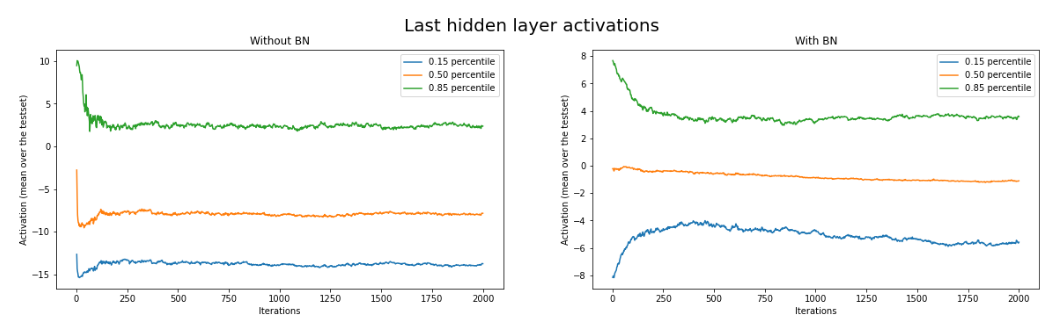
\includegraphics[width=0.9\textwidth]{images/batch_normalization_effect.png}
	\captionof{figure}{So sánh quá trình huấn luyện có và không có Batch Normalization. Mạng sử dụng BN hội tụ nhanh hơn nhiều và đạt được độ chính xác cao hơn so với mạng không sử dụng BN.}
	\label{fig:batch_norm_effect}
\end{center}

\subsubsection{Biến thể và Thách thức của Batch Normalization}
Mặc dù BN rất hiệu quả, nó không phải là “thuốc tiên” cho mọi tình huống. Một số hạn chế và biến thể đã được phát triển:

\paragraph{Hạn chế:}
\begin{itemize}
	\item BN phụ thuộc vào kích thước batch đủ lớn để ước lượng thống kê ổn định. Khi batch size nhỏ (như trong các mô hình segmentation hoặc few-shot learning), BN trở nên kém hiệu quả.
	\item Trong mô hình RNN, sự thay đổi thống kê qua thời gian khiến BN khó áp dụng trực tiếp.
\end{itemize}

\paragraph{Các biến thể:}
\begin{description}
	\item[Layer Normalization (LN):] Chuẩn hóa theo \textit{các đặc trưng} (features) của từng mẫu, thay vì theo batch. Được dùng nhiều trong Transformer.
	\item[Instance Normalization (IN):] Chuẩn hóa từng ảnh độc lập, phổ biến trong các bài toán style transfer.
	\item[Group Normalization (GN):] Chuẩn hóa theo từng nhóm kênh (groups of channels), cân bằng giữa BN và LN, hiệu quả khi batch nhỏ.
\end{description}

\subsection{Dropout: Chống Quá khớp bằng cách "Quên" Ngẫu nhiên}
\label{subsec:dropout}
\textbf{Vấn đề:} Quá khớp (overfitting) là một trong những thách thức lớn nhất trong học sâu. Một mô hình bị quá khớp khi nó học "thuộc lòng" các đặc điểm của tập huấn luyện, bao gồm cả nhiễu, và do đó hoạt động rất kém trên dữ liệu mới. Điều này đặc biệt nghiêm trọng ở các lớp kết nối đầy đủ (fully-connected layers), nơi số lượng tham số là rất lớn.

\textbf{Giải pháp:} Dropout \cite{Srivastava2014} là một kỹ thuật chính quy hóa đơn giản nhưng cực kỳ hiệu quả. Ý tưởng của nó là: trong quá trình huấn luyện, hãy \textbf{ngẫu nhiên "tắt" (drop) một số nơ-ron} ở mỗi bước.

\subsubsection{Cơ chế Hoạt động}
\label{subsubsec:dropout_mechanism}
\begin{itemize}
	\item \textbf{Trong quá trình Huấn luyện:} Tại mỗi lần forward pass, mỗi nơ-ron trong một lớp có Dropout sẽ có xác suất $p$ (dropout rate, ví dụ: $p=0.5$) bị "tắt". Điều này có nghĩa là output của nó sẽ được đặt bằng 0.
	\item \textbf{Trong quá trình Suy luận (Inference/Testing):} Để đảm bảo rằng output có cùng một thang độ (scale) như khi huấn luyện, có hai phương pháp phổ biến:
	\begin{enumerate}
		\item \textbf{Inverted Dropout (phổ biến nhất):} Trong quá trình huấn luyện, output của các nơ-ron không bị "tắt" sẽ được nhân với $1/(1-p)$. Bằng cách này, quá trình suy luận không cần phải làm gì cả; tất cả các nơ-ron đều được sử dụng.
		\item \textbf{Phương pháp gốc:} Trong quá trình suy luận, tất cả các nơ-ron đều được sử dụng, nhưng output của toàn bộ lớp sẽ được nhân với $(1-p)$.
	\end{enumerate}
\end{itemize}

\begin{mdframed}[style=infobox]
	\textbf{Trực giác: Ngăn chặn sự "Đồng phụ thuộc"}
	
	Khi một mạng được huấn luyện bình thường, các nơ-ron có thể phát triển sự "đồng phụ thuộc" (co-adaptation) phức tạp. Tức là, một nơ-ron có thể học cách sửa lỗi cho các nơ-ron khác. Điều này làm cho mô hình trở nên mong manh.
	
	Dropout phá vỡ sự đồng phụ thuộc này. Vì một nơ-ron không thể biết được "đồng đội" nào của nó sẽ bị tắt ở bước tiếp theo, nó buộc phải học các đặc trưng mạnh mẽ và hữu ích một cách độc lập.
	
	Một cách nhìn khác là: tại mỗi bước huấn luyện, Dropout tạo ra một kiến trúc mạng "mỏng" hơn một cách ngẫu nhiên. Việc huấn luyện trên một tập hợp lớn các mạng con khác nhau này có tác dụng tương tự như việc "ensemble" (kết hợp) nhiều mô hình, một kỹ thuật rất mạnh để cải thiện khả năng tổng quát hóa.
\end{mdframed}

\subsubsection{Biến thể của Dropout}
Sau khi Dropout ra đời, nhiều biến thể đã được đề xuất để phù hợp với từng loại kiến trúc:

\begin{itemize}
	\item \textbf{Spatial Dropout:} Thay vì tắt ngẫu nhiên từng nơ-ron, toàn bộ \textit{kênh đặc trưng} (feature map) được tắt cùng lúc. Phù hợp với CNN vì các giá trị trong cùng một feature map có tính tương quan cao.
	\item \textbf{DropBlock:} Một phiên bản có cấu trúc hơn của Spatial Dropout, tắt các khối (block) vuông liên tiếp trong feature map, giúp mạng học các đặc trưng bối cảnh rộng hơn.
	\item \textbf{Monte Carlo Dropout:} Giữ Dropout hoạt động cả trong giai đoạn suy luận để ước lượng độ bất định (uncertainty estimation), được xem như một xấp xỉ Bayesian của mạng nơ-ron.
\end{itemize}

\paragraph{Tương tác với Batch Normalization:}
Dropout và BN đôi khi xung đột nhẹ — BN chuẩn hóa theo thống kê batch, trong khi Dropout làm thay đổi thống kê đó ngẫu nhiên. 
Do đó, trong nhiều mô hình hiện đại (như ResNet, EfficientNet), Dropout được áp dụng \textit{sau BN và chỉ ở phần classifier cuối}.

Dropout thường được áp dụng cho các lớp kết nối đầy đủ, nơi nguy cơ overfitting là cao nhất. Việc áp dụng nó cho các lớp tích chập ít phổ biến hơn và thường sử dụng các biến thể như Spatial Dropout.

\subsection{Data Augmentation: Sáng tạo Dữ liệu để Tổng quát hóa}
\label{subsec:data_augmentation}
\textbf{Vấn đề:} Hiệu năng của các mô hình học sâu phụ thuộc rất nhiều vào số lượng và sự đa dạng của dữ liệu huấn luyện. Tuy nhiên, việc thu thập và gán nhãn dữ liệu mới là một quá trình tốn kém và mất thời gian.

\textbf{Giải pháp:} \textbf{Tăng cường dữ liệu (Data Augmentation)} là một tập hợp các kỹ thuật để tạo ra các mẫu dữ liệu huấn luyện "mới" từ dữ liệu hiện có bằng cách áp dụng các phép biến đổi hợp lý. Mục tiêu là dạy cho mô hình rằng một đối tượng vẫn là chính nó, dù được nhìn dưới các điều kiện hơi khác nhau.

\subsubsection{Các Kỹ thuật Tăng cường Phổ biến}
\label{subsubsec:augmentation_techniques}
Đây là một lĩnh vực rất sáng tạo, với nhiều kỹ thuật khác nhau, có thể được chia thành các nhóm chính:
\begin{description}
	\item[Biến đổi Hình học:] Thay đổi cấu trúc không gian của ảnh.
	\begin{itemize}
		\item \textbf{Lật (Flipping):} Lật ảnh theo chiều ngang (phổ biến nhất), và đôi khi theo chiều dọc.
		\item \textbf{Cắt cúp ngẫu nhiên (Random Cropping):} Cắt ra một vùng ngẫu nhiên từ ảnh gốc (thường sau khi đã thay đổi kích thước một chút). Đây là kỹ thuật cực kỳ hiệu quả.
		\item \textbf{Xoay (Rotation), Dịch chuyển (Translation), Co giãn (Scaling), và Cắt xiên (Shear):} Áp dụng các phép biến đổi affine ngẫu nhiên.
	\end{itemize}
	\item[Biến đổi Quang học/Màu sắc:] Thay đổi các giá trị pixel mà không làm thay đổi cấu trúc hình học.
	\begin{itemize}
		\item \textbf{Color Jitter:} Thay đổi ngẫu nhiên độ sáng (brightness), độ tương phản (contrast), độ bão hòa (saturation), và sắc độ (hue) của ảnh.
	\end{itemize}
	\item[Các Kỹ thuật dựa trên Che khuất (Occlusion-based):]
	\begin{itemize}
		\item \textbf{Cutout / Random Erasing:} Xóa một vùng hình chữ nhật ngẫu nhiên trong ảnh và lấp đầy nó bằng giá trị 0 hoặc một giá trị ngẫu nhiên. Điều này buộc mạng phải học từ bối cảnh và không quá phụ thuộc vào một đặc trưng nổi bật duy nhất.
	\end{itemize}
	\item[Các Kỹ thuật Trộn ảnh (Mixing Images):]
	\begin{itemize}
		\item \textbf{Mixup:} Tạo ra một ảnh mới bằng cách trộn hai ảnh theo một tỷ lệ ngẫu nhiên: $I_{new} = \lambda I_1 + (1-\lambda) I_2$. Nhãn của ảnh mới cũng được trộn theo cùng tỷ lệ.
		\item \textbf{CutMix:} Cắt một vùng từ một ảnh và dán nó vào một ảnh khác. Nhãn cũng được trộn theo tỷ lệ diện tích.
	\end{itemize}
\end{description}

\begin{center}
	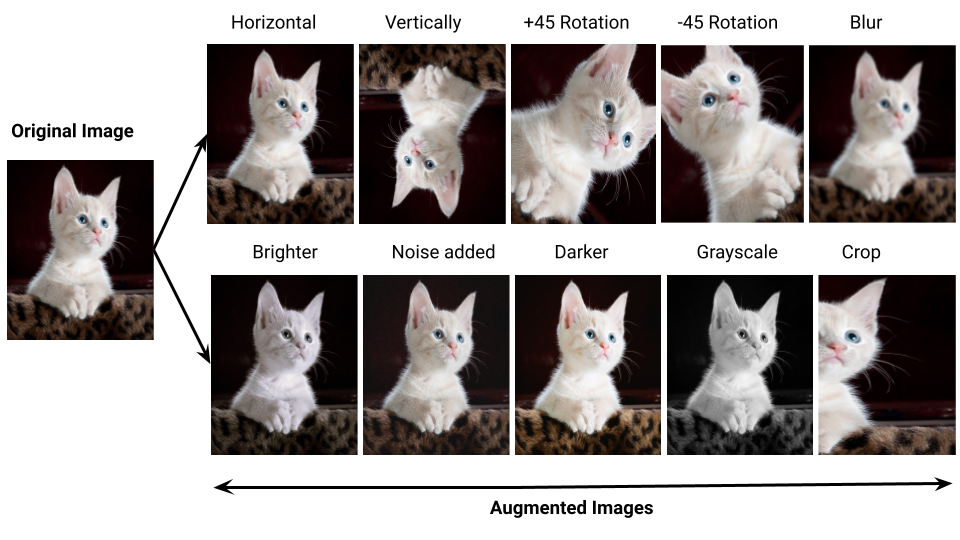
\includegraphics[width=1.0\textwidth]{images/data_augmentation_examples.png}
	\captionof{figure}{Ví dụ về các kỹ thuật Data Augmentation khác nhau được áp dụng trên cùng một ảnh gốc: Lật ngang, Cắt cúp và co giãn ngẫu nhiên, Thay đổi màu sắc (Color Jitter), và Cutout.}
	\label{fig:data_augmentation_examples}
\end{center}

\subsubsection{Các Phương pháp Tăng cường Tự động}
Các kỹ thuật cổ điển yêu cầu chuyên gia chọn thủ công các phép biến đổi. 
Gần đây, các phương pháp học tự động chiến lược tăng cường đã trở thành xu hướng:

\begin{itemize}
	\item \textbf{AutoAugment (2019):} Sử dụng Reinforcement Learning để tìm ra tập hợp phép biến đổi tối ưu cho một bộ dữ liệu cụ thể (như CIFAR-10 hoặc ImageNet).
	\item \textbf{RandAugment (2020):} Giảm không gian tìm kiếm bằng cách chỉ điều khiển hai siêu tham số: số lượng phép biến đổi và độ mạnh của chúng.
	\item \textbf{TrivialAugment (2021):} Một biến thể cực kỳ đơn giản nhưng hiệu quả, chọn ngẫu nhiên một phép biến đổi từ danh sách cố định mà không cần tối ưu thêm.
\end{itemize}


Việc lựa chọn và kết hợp các kỹ thuật tăng cường dữ liệu là một bước quan trọng trong việc thiết kế một pipeline huấn luyện thành công. Các phương pháp hiện đại như AutoAugment và RandAugment thậm chí còn sử dụng các thuật toán để tự động tìm ra các chiến lược tăng cường dữ liệu tối ưu cho một bộ dữ liệu cụ thể.

\subsection{Tổng kết và So sánh}
Ba kỹ thuật trên có thể được xem như ba trụ cột giúp mạng học sâu hiện đại thực sự khả thi:
\begin{itemize}
	\item \textbf{Batch Normalization} giúp việc huấn luyện ổn định và nhanh chóng.
	\item \textbf{Dropout} giúp giảm phương sai của mô hình và cải thiện khả năng tổng quát.
	\item \textbf{Data Augmentation} mở rộng không gian dữ liệu, giảm bias và tăng khả năng chống nhiễu.
\end{itemize}

\begin{table}[h!]
	\centering
	\caption{So sánh vai trò và đặc tính của các kỹ thuật chính quy hóa / tối ưu phổ biến}
	\begin{tabular}{lccc}
		\toprule
		\textbf{Kỹ thuật} & \textbf{Mục tiêu chính} & \textbf{Tác động} & \textbf{Áp dụng phổ biến} \\
		\midrule
		Batch Normalization & Ổn định gradient & Tăng tốc hội tụ & CNN, Transformer \\
		Dropout & Giảm phương sai mô hình & Chống overfitting & MLP, Classifier head \\
		Data Augmentation & Mở rộng dữ liệu & Tăng khả năng tổng quát & Thị giác máy tính \\
		\bottomrule
	\end{tabular}
\end{table}

\section*{Tài liệu tham khảo}
\begin{itemize}
	\item[1] Ioffe, S.,\& Szegedy, C. (2015). Batch normalization: Accelerating deep network training by reducing internal covariate shift. In \textit{International conference on machine learning (ICML)}. (Paper gốc giới thiệu Batch Normalization).
	\item[2] Srivastava, N., Hinton, G., Krizhevsky, A., Sutskever, I.,\& Salakhutdinov, R. (2014). Dropout: a simple way to prevent neural networks from overfitting. \textit{The journal of machine learning research}, 15(1), 1929-1958. (Paper gốc giải thích chi tiết về kỹ thuật Dropout).
	\item[3] Shorten, C.,\& Khoshgoftaar, T. M. (2019). A survey on image data augmentation for deep learning. \textit{Journal of Big Data}, 6(1), 60. (Một bài tổng quan chi tiết về các kỹ thuật Data Augmentation).
	\item[4] DeVries, T.,\& Taylor, G. W. (2017). Improved regularization of convolutional neural networks with cutout. \textit{arXiv preprint arXiv:1708.04552}. (Giới thiệu kỹ thuật Cutout).
	\item[5] Zhang, H., Cisse, M., Dauphin, Y. N.,\& Lopez-Paz, D. (2017). mixup: Beyond empirical risk minimization. \textit{arXiv preprint arXiv:1710.09412}. (Giới thiệu kỹ thuật Mixup).
	\item[6] Yun, S., Han, D., Oh, S. J., Chun, S., Choe, J.,\& Yoo, Y. (2019). Cutmix: Regularization strategy to train strong classifiers with localizable features. In \textit{Proceedings of the IEEE/CVF international conference on computer vision (ICCV)}. (Giới thiệu kỹ thuật CutMix).
	\item[7] Cubuk, E. D., Zoph, B., Shlens, J.,\& Le, Q. V. (2019). Randaugment: Practical automated data augmentation with a reduced search space. In \textit{Proceedings of the IEEE/CVF Conference on Computer Vision and Pattern Recognition Workshops (CVPRW)}. (Giới thiệu RandAugment, một phương pháp tăng cường dữ liệu tự động hiệu quả).
\end{itemize}